% !TeX spellcheck = pt

%% ************************************************
%% Universidade Nova de Lisboa
%% NOVA Information Management School
%% Computação em Estatística e Gestão de Informação
%% Júlio Caineta, 2015
%% ************************************************
\documentclass[addpoints]{exam}
\usepackage[utf8]{inputenc}
\usepackage{amsmath}
\usepackage[portuguese]{babel}
\usepackage[hidelinks,pdfusetitle]{hyperref}
\author{Júlio Caineta}
\title{CEGI 2015/2016 - Exame 1ª Época - Versão A}
\usepackage{lastpage}
\usepackage{minted}
\usepackage{gensymb}
\usepackage{wrapfig}
\usepackage{tabulary}
\usepackage{graphicx}
\usepackage{xfrac}
\usepackage{multirow}
\usepackage{caption}
\usepackage{etoolbox}
\usepackage[phantomtext]{dashundergaps}
%\usepackage{color}
%\usepackage{draftwatermark}
%\SetWatermarkText{RASCUNHO}
%\SetWatermarkScale{3}
%\SetWatermarkLightness{0.7}
\cfoot{Página \thepage\ de \pageref{LastPage}}
\renewcommand{\solutiontitle}{\noindent\textbf{Solução:}\par\noindent}
\pointpoints{valor}{valores}
\pointsinrightmargin
\bracketedpoints
\marginpointname{ val.}
\renewcommand*\half{.5}
\hqword{Pergunta}
\hpgword{Página}
\hpword{Cotação}
\hsword{Cotação obtida}
\htword{Total}
\newminted{r}{autogobble}
\newmintinline{r}{}
\newtoggle{sol}

\toggletrue{sol}
 
\iftoggle{sol}{
	\printanswers
	%\shadedsolutions
}


%\titlegraphic{}

\begin{document}
	
\noindent\begin{minipage}{0.2\textwidth}% adapt widths of minipages to your needs
	
\includegraphics[width=2cm]{logo.png}
\end{minipage}
\hfill
\begin{minipage}{0.8\textwidth}
	\begin{center}
		\textsc {\small NOVA IMS -- Universidade Nova de Lisboa} \\
		\textsc {Computação em Estatística e Gestão de Informação \\ 2º Semestre 2015/16}
	\end{center}
\end{minipage}

\begin{center}
%	\vspace{5mm} \\
	{\large Exame 1ª Época -- Versão A -- 27/06/2016}
\end{center}
 
\vspace{5mm}
\makebox[\textwidth]{Número: \underline{\phantom{XXXXXXXX}} Nome:\enspace\hrulefill}
\vspace{5mm}

{{\large\textbf{Leia, por favor, com atenção:}}
\begin{enumerate}
	\item Este exame deverá ser realizado no enunciado, sem acesso a um computador.
	\item Poderá consultar o formulário dado em anexo ao exame.
	\item É proibido o uso de qualquer outro material de apoio (livros, apontamentos, telemóvel), assim como a troca de qualquer informação com os colegas.
	\item A entrega do exame e a saída da sala só são possíveis no final do exame.
	\item Deverá escrever o seu nome, número e curso no cabeçalho desta folha.
	\item As respostas às questões deverão ser dadas, exclusivamente, na folha do enunciado, no espaço reservado para tal. Estas respostas deverão ser apenas código em \textbf{R}.
	\item Não é necessário escrever o resultado do código, mas apenas o código em si.
	\item O não cumprimento de alguma das regras conduzirá à anulação do exame.
	\item A duração do exame é de 75 minutos.
\end{enumerate}

\vspace{10mm}

\begin{questions}
	% funções
	\question Uma das vantagens em utilizar uma linguagem de programação interpretada como o \textbf{R} é a interactividade com o utilizador, que, por sua vez, é útil na resolução de problemas de matemática.
	
	\begin{parts}
		\part[2] A regressão é uma das técnicas utilizadas em modelação estatística e econometria. Alguns desses modelos são definidos por equações quadráticas que, tipicamente, têm a forma ilustrada na \autoref{eq:qua}:
		
		\begin{equation}
		\label{eq:qua}
			ax^2+bx+c=0
		\end{equation}
		
		onde $x$ representa um número desconhecido, e $a$, $b$, e $c$ são os coeficientes da equação e representam números conhecidos, tal que $a \neq 0$. \textbf{Se $a = 0$}, então a equação é linear, e não quadrática.
		
		Uma forma de resolver uma equação quadrática é através da fórmula resolvente (\autoref{eq:fr}).
		
		\begin{equation}
		\label{eq:fr}
			x = \frac{-b \pm \sqrt{b^2 - 4 ac}}{2a}
		\end{equation}
		
		\iftoggle{sol}{}{\pagebreak}
		Escreva uma função que permita resolver uma equação quadrática, usando a fórmula resolvente. A função deve devolver \rinline{NULL} caso os coeficientes não sejam de uma equação quadrática.\iftoggle{sol}{}{~\makeemptybox{2.5in}}
		
		\iftoggle{sol}{\pagebreak}{}
			\begin{solution}
				\begin{rcode}
					FormulaResolvente = function (A, B, C) {
						if (A == 0) {
							return (NULL)
						} else {
							zeros = c()
							num = sqrt(B ^ 2 - 4 * A * C)
							den = 2 * A
							zeros[1] = (-B + num) / den
							zeros[2] = (-B - num) / den
							return (zeros)
						}
					}
				\end{rcode}
			\end{solution}
			
		\part[2] No exercício anterior, procurava-se o valor de uma variável desconhecida. O \textbf{R} também pode ser usado para encontrar os valores de múltiplas variáveis desconhecidas, desde que se trate de um \textit{problema bem-posto}. A função \rinline{solve()} serve para resolver um sistema de equações linear.
		
		Escreva o código necessário que permita resolver o seguinte sistema de equações.
		
		\begin{align*}
			\left\{\begin{matrix}
			3x & + & 0.14y & = & \pi \\
			2.71x & - & 0.82y & - & 0.82z & = & 0 \\
			y & + & z & = & 3
			\end{matrix}\right.
		\end{align*}\iftoggle{sol}{}{~\makeemptybox{1.5in}}
		
		\begin{solution}
			\begin{rcode}
				> coefs = matrix(c(3, .14, 0, 2.71, -0.82, -0.82, 0, 1, 1),
				+ nrow=3, ncol=3, byrow=TRUE)
				> ys = c(pi, 0, 3)
				> solve(coefs, ys)
				[1] 0.90774908 2.98818158 0.01181842
			\end{rcode}
		\end{solution}
		
	\end{parts}
	
	% 2. Converter ciclos
	
	\question A linguagem de programação \textbf{R} é compatível com o paradigma de programação funcional. Neste paradigma, é dado um maior ênfase à \textbf{utilização de funções}, em contraste à programação imperativa, que privilegia mudanças no estado do programa. Geralmente, a programação funcional tem ainda a vantagem de ser possível escrever a mesma funcionalidade em menos código.
	
	\begin{parts}
		
		\part[2] Considere que a variável \rinline{islands} é um ~\rinline{vector} de números inteiros, contendo as áreas das maiores massas de terra. Cada posição do vector tem também um nome associado.
		
		\begin{rcode}
			# Excerto do vector islands
			> islands
			Africa       Antarctica             Asia        Australia     Axel Heiberg 
			11506             5500            16988             2968               16 
			Baffin            Banks           Borneo          Britain          Celebes 
			184               23              280               84               73 
		\end{rcode}
		
		\pagebreak
		Analise o seguinte bloco de código.
		
		\begin{minted}[linenos=true, autogobble]{r}
			i = 1
			s = 0
			while (i < length(islands)) {
				if ( islands[i] > sd(islands)) {
					s = islands[i] + s
				}
				i = i + 1
			}
			# para a sua solução, não precisa de considerar a seguinte linha
			names(s) = NULL
		\end{minted}
			
		\begin{rcode}
			> s
			[1] 53924
		\end{rcode}

		
		Reescreva-o sem usar uma estrutura iterativa.\iftoggle{sol}{}{~\makeemptybox{1in}}
		
		\begin{solution}
			\begin{rcode}
				sum(islands[islands > sd(islands)])
			\end{rcode}
		\end{solution}
		
		\part[3] Analise o seguinte bloco de código.
		
		\begin{minted}[linenos=true, autogobble]{r}
			s = c()
			for (num in rnorm(10)) {
				
				if(num > 0) {
					s = c(s, "+")
				} else {
					if(num == 0) {
						s = c(s, "0")
					} else {
					s = c(s, "-")
					}
				}
			}
		\end{minted}
		
		\begin{rcode}	
			> s
			[1] "-" "+" "+" "-" "-" "-" "+" "+" "+" "+"
		\end{rcode}
		
		Reescreva-o sem usar uma estrutura iterativa.\iftoggle{sol}{}{~\makeemptybox{1in}}
		
		\begin{solution}
			\begin{rcode}
				sapply(rnorm(10), function(x) if(x > 0) {"+"} else if (x == 0) {'0'} else {'-'})
			\end{rcode}
		\end{solution}
		
	\end{parts}
	
	\iftoggle{sol}{}{\pagebreak}
	% 3. Manipulação
	
	% a) ler ficheiro
	\question Em \textbf{R} é fácil trabalhar com ficheiros de diferentes formatos e manipular a informação contida neles.
	
	\begin{parts}
		\part[1\half] Considere o seguinte conteúdo de um ficheiro de nome \textit{pauta.dat}:
		
			\begin{minted}[autogobble]{text}
				Nome;AM2;CEGI;DP1;Est1;ISC;Mrkt
				Regina;12,1;14,4;15,2;11,7;10,0;15,5
				Dudu;8,2;6,6;12,3;9,9;13,1;16,7
				Gioberte Nelson;13,3;13,3;13,3;13,3;13,3;13,3
				Enzo;18,0;19,0;20,0;17,0;19,0;15,0
				Valter Disnei;10,0;11,1;12,2;13,3;14,4;15,5
			\end{minted}
			
			Escreva o código necessário para guardar o conteúdo deste ficheiro num \rinline{data.frame}, com 5 linhas e 7 colunas, guardado na variável \rinline{pauta}.\iftoggle{sol}{}{~\makeemptybox{0.9in}}
			
			\begin{solution}
				\begin{rcode}
					pauta = read.table(file="pauta.dat", header=TRUE, sep=";", dec=",")
				\end{rcode}
			\end{solution}
		
		% b) manipulação de dados	
		\part[2\half] Considere a variável \rinline{pauta}, contendo a tabela da alínea anterior. Essa tabela contém as notas de 5 alunos em 6 disciplinas. Modifique-a, acrescentando as seguintes colunas:
		
		\begin{description}
			\item[dif] Indica se a diferença entre as notas a CEGI e a AM2 é ou não superior a 2 valores.
			\item[med] O valor da média ponderada das notas de CEGI e de ISC, dando um peso de 70\% a CEGI e 30\% a ISC.
		\end{description}
		
		Não utilize estruturas iterativas.\iftoggle{sol}{}{~\makeemptybox{1in}}
		
		\begin{solution}
			\begin{rcode}
				pauta = transform(pauta, dif = abs(CEGI - AM2) > 2,
							 med = CEGI * 0.7 + ISC * 0.3)
			\end{rcode}
			\textbf{Nota}: A não utilização da função \rinline{abs()} não foi penalizada.
		\end{solution}
			
	\end{parts}
	
	% 4. Gráficos
	
	\question Em \textbf{R} existe também um vasto leque de funções para criar gráficos, sendo relativamente fácil produzir imagens de elevada qualidade. Nas próximas questões, analise os gráficos e escreva o código necessário para os reproduzir.
	
	\begin{parts}
		\part[1\half] Escreva o código necessário para reproduzir o gráfico na \autoref{graf:hist}, em que \rinline{x = rnorm(100)}.
		% a) histograma + curva de densidade
		\begin{figure}[!htb]
			\centering
			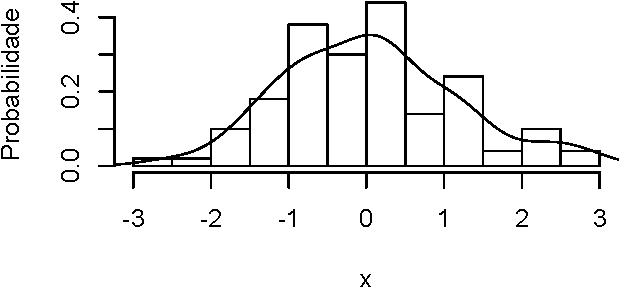
\includegraphics[width=10cm]{hist-crop}
			\caption{}
			\label{graf:hist}
		\end{figure}\iftoggle{sol}{}{~\makeemptybox{1in}}

		\begin{solution}
			\begin{rcode}
				hist(x, main = "", ylab = "Probabilidade", probability = TRUE)
				lines(density(x))
			\end{rcode}
		\end{solution}
		
		\iftoggle{sol}{\pagebreak}{}
		
		\part[1\half] Escreva o código necessário para reproduzir o gráfico na \autoref{graf:barplot}. Considere as seguintes linhas de código.
		
		\begin{rcode}
			> y = runif(10, 0, 20)
			> mean(y)
			[1] 10.49255
		\end{rcode}
		
		% b) barplot + linha com a média
		\begin{figure}[!htb]
			\centering
			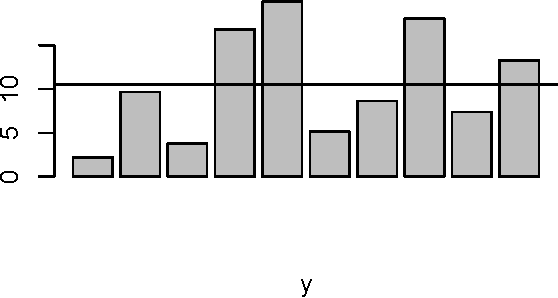
\includegraphics[width=10cm]{barplot-crop}
			\caption{}
			\label{graf:barplot}
		\end{figure}\iftoggle{sol}{}{~\makeemptybox{1in}}
		
		\begin{solution}
			\begin{rcode}
				barplot(y, xlab='y')
				abline(h=mean(y))
			\end{rcode}
		\end{solution}
		
	\end{parts}
	
	% 5. Explicar o código.
	
	\question[4] O \rinline{data.frame rock} contém valores de quatro propriedades de 48 amostras de rocha. As seguintes instruções executadas em \textbf{R} fornecem uma noção sobre a estrutura deste objecto.
	
	\begin{rcode}
		# primeiras 5 linhas do data.frame rock
		rock
		area     peri     shape   perm
		1   4990 2791.900 0.0903296    6.3
		2   7002 3892.600 0.1486220    6.3
		3   7558 3930.660 0.1833120    6.3
		4   7352 3869.320 0.1170630    6.3
		5   7943 3948.540 0.1224170   17.1
	\end{rcode}
		
	\iftoggle{sol}{}{\pagebreak}
		
	\begin{rcode}
		> str(rock)
		'data.frame':	48 obs. of  4 variables:
		$ area : int  4990 7002 7558 7352 7943 7979 9333 8209 8393 6425 ...
		$ peri : num  2792 3893 3931 3869 3949 ...
		$ shape: num  0.0903 0.1486 0.1833 0.1171 0.1224 ...
		$ perm : num  6.3 6.3 6.3 6.3 17.1 17.1 17.1 17.1 119 119 ...
	\end{rcode}
	
	Explique, por palavras suas, o que se pretende encontrar com o seguinte bloco de código, e como isso é conseguido.
	
	\begin{minted}[linenos=true, autogobble]{r}
		qs = apply(rock, 2, quantile, .25)
		rock[apply(rock, 1, function(x) sum(x > qs) == 2), ]
	\end{minted}
	
	\iftoggle{sol}{}{\makeemptybox{3in}}
	
	\begin{solution}
			Pretende-se encontrar quais são as amostras em que o valor de duas das suas variáveis são maiores que o respectivo primeiro quartil.
			
			Na primeira linha, o \rinline{data.frame rock} é percorrido pelas suas colunas, calculando, para cada uma delas, o valor do primeiro quartil.
			
			Na segunda linha, o mesmo \rinline{data.frame} é percorrido pelas linhas, avaliando-se uma função anónima em cada linha. Esta função compara (verifica se é maior) o valor de cada variável numa linha com o respectivo quartil, calculado na linha anterior.
			
			O resultado dessa comparação é um vector de valores lógicos. O número de valores que são \rinline{TRUE} é calculado pela função \rinline{sum}, sendo feita a conversão de lógico para inteiro implicitamente. De seguida, verifica-se se esta contagem é igual a dois, retornando o valor lógico correspondente.
			
			Por último, esse vector de valores lógicos é usado para seleccionar apenas as amostras (linhas) em que a condição pretendida é verificada.
	\end{solution}
	
%	\question[3] Considere agora o conjunto de dados \rinline{iris}, contendo informação sobre 150 amostras de flores, acerca de 4 propriedades e a respectiva espécie.
%	
%	Pretende adicionar uma nova amostra ao conjunto existente. A \autoref{amostra} contém os valores das propriedades dessa amostra. Usando a técnica de classificação do vizinho mais próximo, descubra qual é a sua espécie.
%		
%	\begin{table}[h]
%		\centering
%		\begin{tabulary}{0.9\textwidth}{|C|C|C|C|C|}
%			\hline Número do examplar & Comprimento da Sépala & Largura da Sépala & Comprimento da Pétala & Largura da Pétala \\ 
%			\hline Nova amostra & 6,6 & 3,0 & 3,4 & 2,2 \\  
%			\hline
%		\end{tabulary}
%		\caption{Características da nova amostra de flor Iris.}
%		\label{amostra}
%	\end{table}
%		
%	Assuma que cada característica tem o mesmo peso. Utilize a distância de Mahalanobis, já implementada na função \rinline{mahalanobis}, para encontrar o vizinho mais próximo.
%	
%	\begin{solution}
%		\begin{rcode}
%			> am = c(6.6, 3, 3.4, 2.2)
%			> iris$Species[which.min(mahalanobis(iris[,-5], am, cov(iris[,-5])))]
%			[1] setosa
%		\end{rcode}
%	\end{solution}
	
\end{questions}

\vspace{10mm}
%\centerline
	\begin{center}
		\gradetable[h][questions]
		\small{\\ \vspace{3mm}(a preencher pelo docente)}
	\end{center}
	
\end{document}